

\section{Metodologia}\label{sec:metodology}
O acompanhamento é pautado nos níveis de SpO$_2$ detectados pelo SMA-oxímetro; com a triagem feita de forma autonoma pelo sistema. graças à sociedade de agentes embarcada no microcontrolador. 
O SMA faz o monitoramento integral do enfermo, mantendo uma rede de apoio e um responsável técnico (médico) cientes de casos críticos. 
O fluxo de interação entre usuários e o SMA está disposto na Figura~\ref{fig:fig1}.

\begin{figure}[H]
  \centering
  \includegraphics[width=0.5\textwidth]{assets/img/interações.png}
  \caption{Diagrama de Interações}
  \label{fig:fig1}
\end{figure}

A medição é feita estabelecendo a comunicação entre os componentes do microcontrolador e o programa AgentSpeak; que é feita pela compilação do \textit{firmware} do Arduino, ARGO \cite{ArgoAgent}, na ChonIDE. A inicialização das percepções do \textit{hardware} também é feita na IDE, pelo botão de \textbf{\textit{Play}}, sendo o valor de saturação padrão 98\%, nível considerado normal em indivíduos saudáveis \cite{collins2015relating}.

Alterações nos níveis de SpO$_2$ podem ser observadas durante a interação do usuário com o teclado LCD, sendo o botão direito responsável pelo incremento e o esquerdo, pelo decremento no percentual de saturação, respectivamente.

O sistema, durante a percepção, baseando-se nos níveis de SpO$_2$ começa a efetuar o diagnóstico inicial e comunicar o quadro de risco correlato à leitura ao agente \textbf{monitor}, que exibe essa informação no console da aplicação. A classificação de risco efetuada pela aplicação é ilustrada na  Tabela~\ref{tab:tabela1}


\begin{table}[ht]
    \centering
    \begin{tabular}{|c|c|c|}
        \hline
        \textbf{Risco} & \textbf{Mínimo (\%)} & \textbf{Máximo (\%)} \\
        \hline
        Normal & 96 & 100 \\ 
        \hline
        Alerta & 90 & 95 \\ 
        \hline
        Crítico & 0 & 89 \\ 
        \hline
    \end{tabular}
    \caption{Indicadores de Risco: SpO$_2$}
    \label{tab:tabela1}
\end{table}

Casos considerados críticos são comunicados ao agente \textbf{mensageiro}, cuja responsabilidade é identificar a rede de apoio atrelada ao paciente e disparar mensagens acerca de seu quadro de saúde. Esse cenário pode ser observado nas Figuras~\ref{fig:fig2} e~\ref{fig:fig3}

\begin{figure}[H]
  \centering
  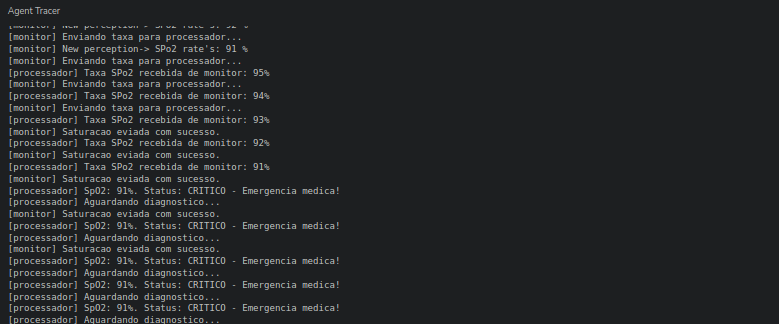
\includegraphics[width=0.7\textwidth]{assets/img/perception.emergency.png}
  \caption{Estado Crítico}
  \label{fig:fig2}
\end{figure}


\begin{figure}[H]
  \centering
  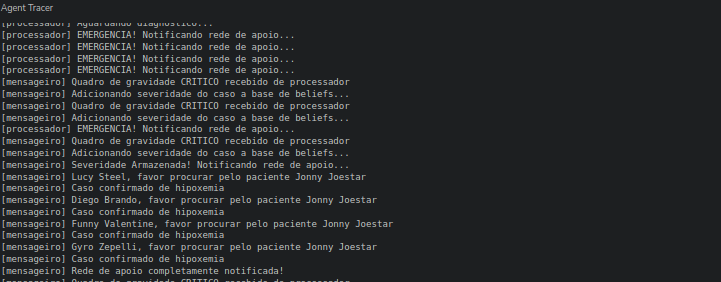
\includegraphics[width=0.7\textwidth]{assets/img/netwokcall.png}
  \caption{Contactando Rede}
  \label{fig:fig3}
\end{figure}

O modelo conceitual da arquitetura de responsabilidade única usado na construção do oxímetro está ilustrado na Figura~\ref{fig:fig4}. 
No diagrama está disposto todo o fluxo de interação e processamento de dados feito pelo oxímetro, desde a etapa de coleta até a mensageria.

\begin{figure}[H]
  \centering
  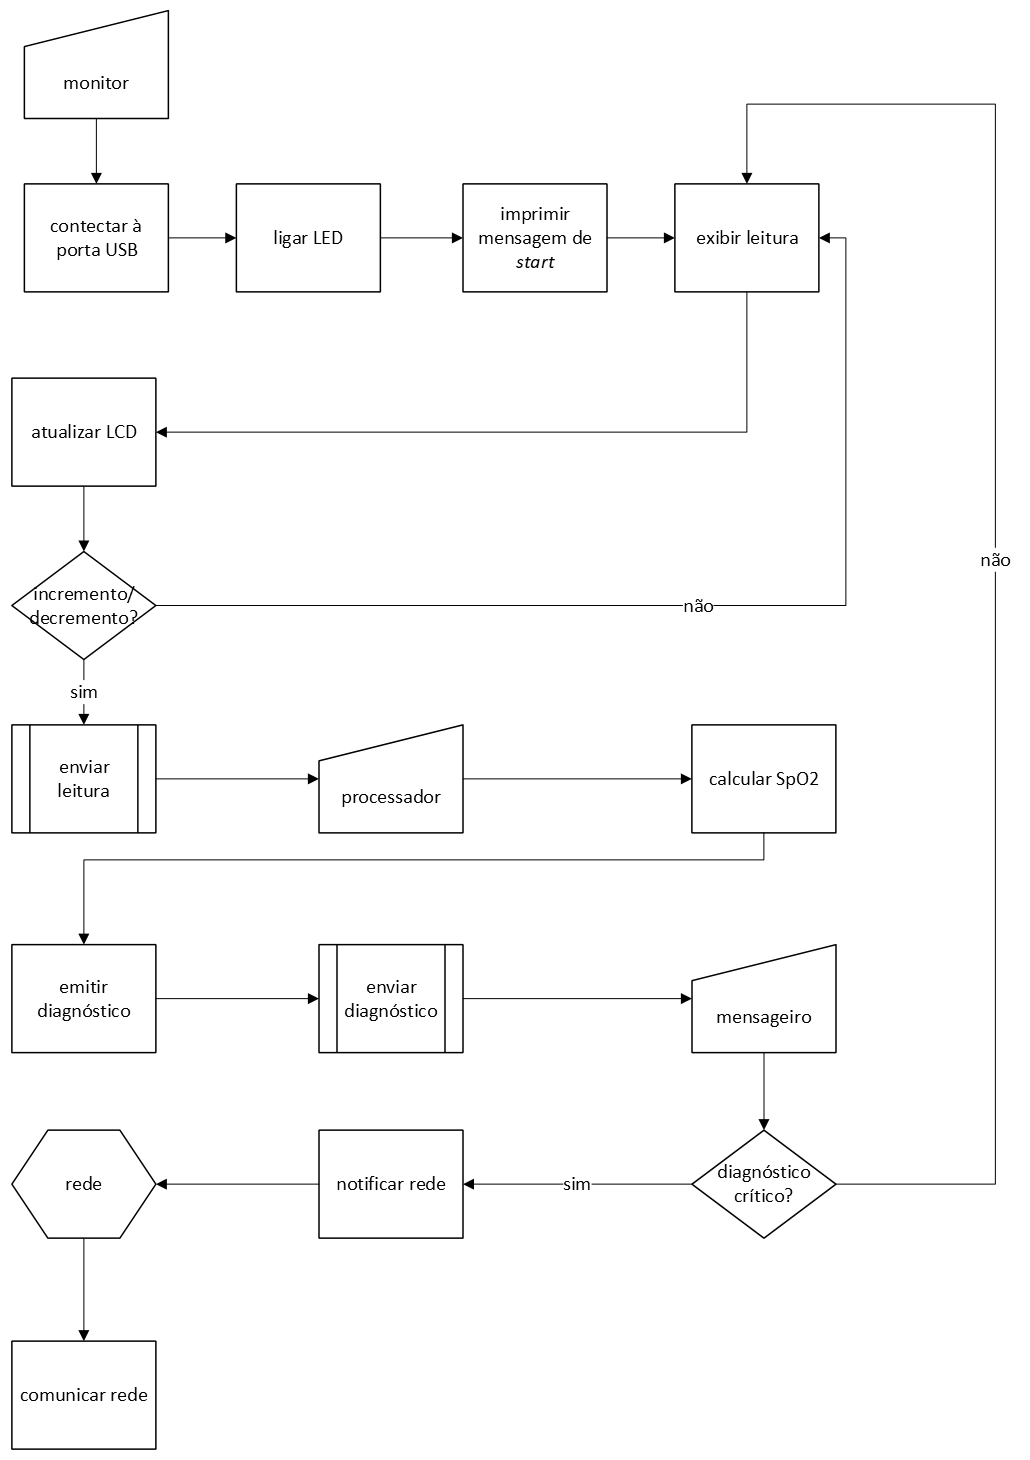
\includegraphics[width=0.7\textwidth]{assets/img/diagrama.png}
  \caption{Arquitetura Conceitual}
  \label{fig:fig4}
\end{figure}

\section{Métodos}\label{sec:methods}
% \section{Métodos}\label{sec:methods}


A presente pesquisa adota uma abordagem avaliativa, a fim de validar o funcionamento do protocolo de comunicação Multi-Agente aplicado à medição dos níveis de saturação periférica de oxigênio (SpO$_2$). O estudo baseia-se na construção de um protótipo funcional de oxímetro, utilizando Arduino UNO, e no desenvolvimento de um sistema lógico de controle e monitoramento escrito na linguagem AgentSpeak, compilado e executado na ferramenta ChonIDE. A coleta de dados ocorre diretamente no protótipo físico, enquanto o processamento e a interpretação das informações são realizados pelo programa denominado \textit{\textbf{Oximeter}}. Essa configuração permite avaliar, de forma objetiva e controlada, a capacidade de comunicação entre hardware e software e a fidelidade das informações apresentadas no console, validando o comportamento esperado do sistema frente às condições experimentais simuladas.


\section{Implementação}\label{sec:deployment}
Nesta pesquisa, foi realizada a construção de um protótipo SMA, embarcado em uma placa Arduino; para aferir a viabilidade do uso de SMAs na construção de oxímetros autônomos. O sistema foi capaz de realizar a coleta ativa dos níveis de SpO$_2$ do paciente, efetuar a classificação de risco e realizar o \textit{broadcast} do diagnóstico em casos considerados graves.

% Para isso, foi construído um protótipo utilizando o microcontrolador Arduino, equipado com um teclado LCD para simulação e controle manual dos níveis de saturação de O$_2$. O dispositivo foi integrado a uma rede de agentes autônomos, desenvolvida na linguagem AgentSpeak com o apoio da plataforma \textbf{ChonIDE}.
% \subsection{Ferramentas}\label{sub:tools}
% \section{Ferramentas} \label{sec:tools}
O protótipo foi equipado com um teclado LCD e três LEDs distintos; sendo o uso do teclado pela necessidade de atualização das crenças do agente monitor, responsáveis pela quantificação dos níveis de SpO$_2$ no sangue. Ademais, o componente também possui saída de dados por meio do visor LCD, para constatação dos dados exibidos na ChonIDE. Os LEDs foram escolhidos para identificar o status do hardware ao carregar o firmware compilado.
A escolha desse ferramental se deu pelo seu baixo custo e amplo suporte aos componentes, tornando a experimentação viável. O aparato descrito pode ser observado na Figura~\ref{fig:fig5}

\begin{figure}[H]
  \centering
  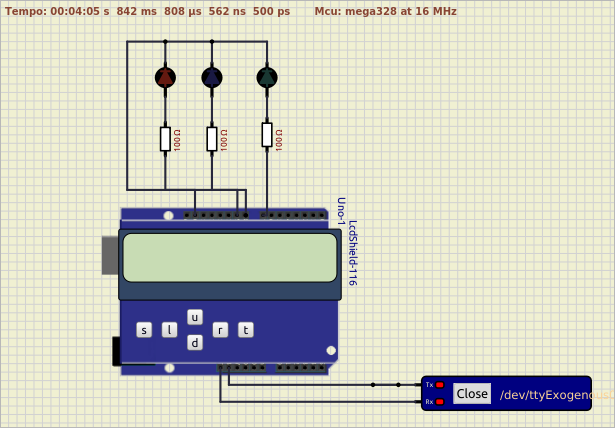
\includegraphics[width=0.7\textwidth]{assets/img/Oximeter.png}
  \caption{Protótipo do Oxímetro. Disponível Blind Review.}
  \label{fig:fig5}
\end{figure}

Já a parte lógica do projeto foi construída em \textit{AgentSpeak} na ChonIDE, para integração com o microcontrolador Arduino, por meio do Javino; durante a compilação do firmware escrito em ArduINO. Oximeter, projeto criado na ChonIDE para esta pesquisa, foi arquitetado seguindo o paradigma Multi-Agente, sendo constituído de quatro camadas de responsabilidade compostas por um agente cada. Assim, há melhor manutenção e escalabilidade ao projeto, seguindo os preceitos arquiteturais do ARGO \cite{pantoja2016argo}.

% \begin{figure}[H]
%   \centering
%   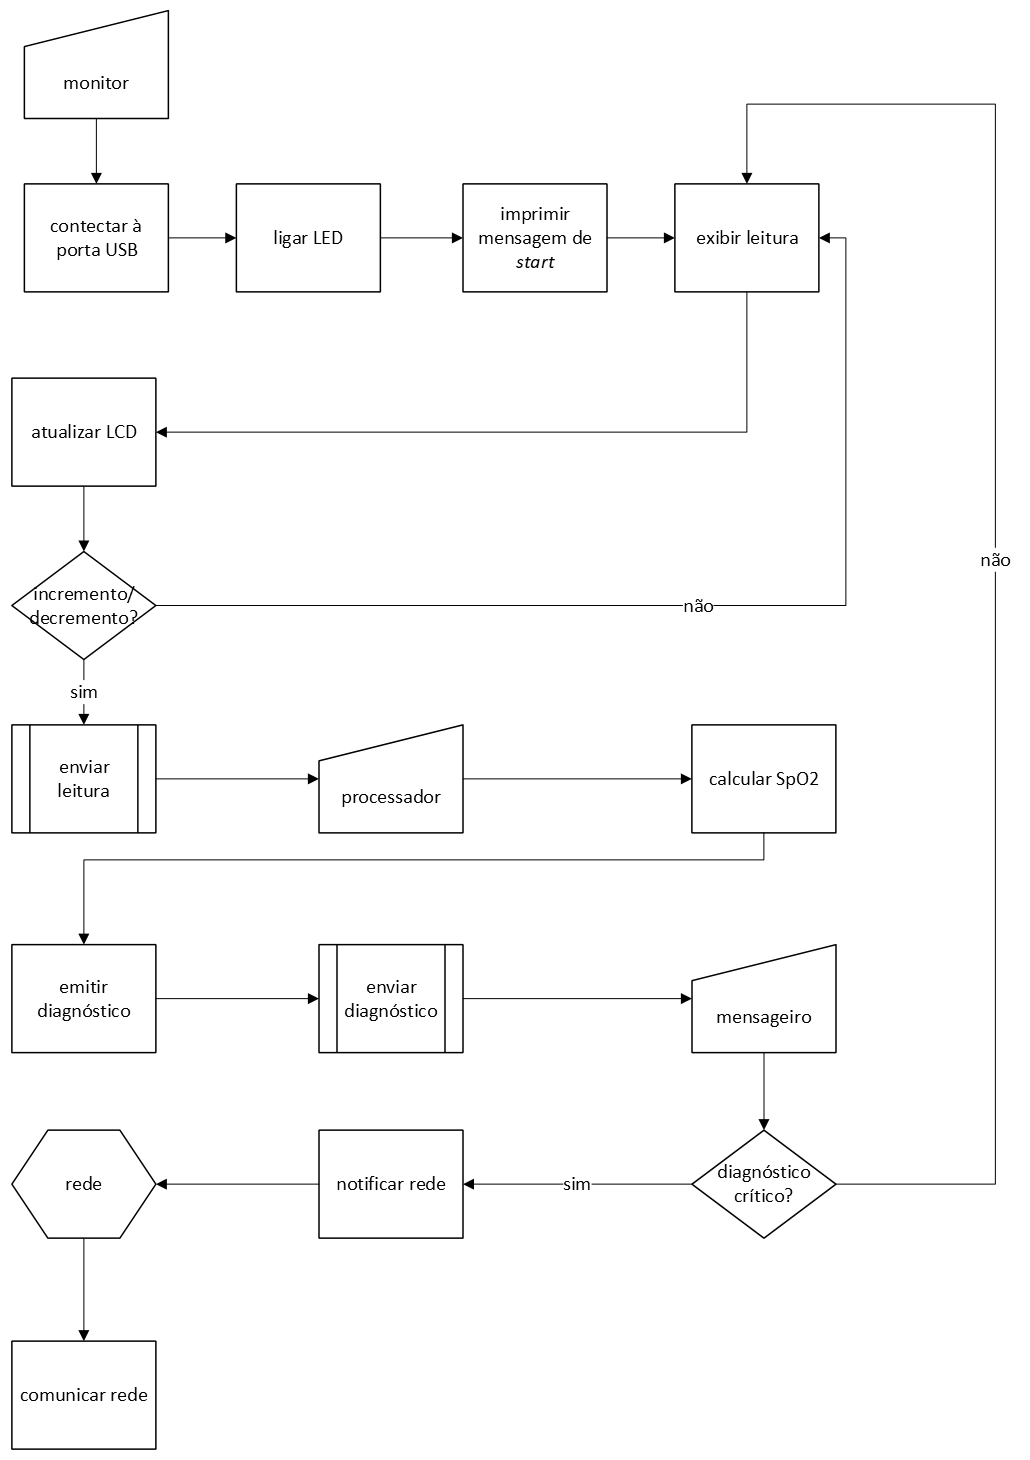
\includegraphics[width=0.9\textwidth]{assets/img/diagrama.png}
%   \caption{Arquitetura Conceitual}
%   \label{fig:fig4}
% \end{figure}
